\documentclass[a4paper]{article}
\usepackage{lrec}
\usepackage{amsmath}
\usepackage{polyglossia}
\usepackage{graphicx}
\usepackage{hyperref}
\hypersetup{
    colorlinks=true,
    linkcolor=blue,
    filecolor=magenta,      
    urlcolor=blue,
}

\setmainfont{FreeSerif}
\setmainlanguage{english}
\setotherlanguages{russian}

\newcommand{\head}[1]{\vspace{0.5em}\emph{#1}\vspace{0.25em}}

\abstract{
	Linguistics predictability is the degree of confidence in which language unit (word, part of speech, etc.) will be the next in the sequence. Experiments have shown that the correct prediction simplifies the perception of a language unit and its integration into the context. As a result of incorrect prediction language processing slows down. Currently, in order to get a measure of the language unit predictability, a neurolinguistic experiment known as cloze task has to be conducted on a large number of participants. Cloze tasks are resource-consuming and are criticized by some researchers as an insufficiently valid measure of predictability. In this paper we compare different language models that attempt simulating human respondents' performance on the cloze task. Using a language model to create cloze task simulations would require significantly less time and conduct studies related to linguistic predictability.
}


\title{Semantic prediction in {R}ussian}

\name{\begin{tabular}{l}Anastasia Nikiforova, Sergey Pletenev, Daria
Sinitsyna, \\
Semen Sorokin, Anastasia Lopukhina, Nicholas Howell\end{tabular}}
\address{National Research University Higher School of Economics \\ Moscow,
Russian Federation}



\begin{document}
\maketitleabstract
\nocite{*}


\section{Introduction}

% TODO: clarify introduction: is this article about semantic
% prediction, or about modeling cloze task performance?
Nowadays language models are the most powerful instrument to transfer knowledge. Mostly pre-trained neural network models are more accurate in any type of tasks. This tendency in language processing - usage of language model (LM) weights as a part of base model weights - took place after word2vec announcing. Today there are three main ways to use pre-trained LM in different natural language processing tasks. 
\begin{itemize}
	\item Use pre-trained LM as universal embedder for text/sentence
	\item Fit pre-trained LM on new data (domain adaptation) and also use as an embedder
	\item Fit pre-trained LM as a part of more complex and specific model
\end{itemize}
It is important to note that the resulting model is very dependent on the quality of the based LM. So a possibility to compare models is also demanded and we propose a new comprehensive way to explore properties of different language models.
Comparing LM is not a new topic. There is a lot of different tasks to measure their quality. It starts with the google analogy task for word2vec \cite{mikolov2013efficient} and now GLUE tasks\cite{Wang2018GLUEAM} are used for these purposes. However, we want to check the generative ability of a different type of LM and compare them to each other.
One of the the key terms in natural language understanding and speech generation is predictability. In cognitive linguistics, it implies a confidence degree of a language unit (word, part of speech, etc.) that can take next place in the sentence (or text). This property of the token in the context is usually measured in terms of the theory of probability, and it also has some well-known probabilistic properties. For example, the sum of the probabilities of all words which can or cannot (in terms of common sense) “continue” the left context is equal to one. A quarter-century ago these assumptions led to the emergence of the first artificial language models (ALM).

Research papers in the field of cognitive science have shown that correct prediction of the next word while reading a sentence simplifies the perception of a language unit and its integration into the context. Incorrect prediction can lead to re-analysis of the context which is why language processing is slowed down. However, the types of dependencies between these two facts are still not well studied.
% TODO: add citations 

Nowadays, in linguistic and cognitive studies, to obtain data describing the probabilistic distribution of lexical units (for a specific context), artificial language models of various architectures are used or cloze tests are conducted on real-life participants. They are asked to replace the missing language item in a sentence. However The cloze test is frequently criticized for lack of coverage. Nevertheless, in terms of common sense, it is a cloze test, which uses the so-called “human” linguistic mechanisms of speech generation to collect the data. The ALM, in contrast, is basically a set of various mathematical algorithms applied to the text corpus.
Our approach is based on the specific Russian corpus manually collected for the purposes of experiments with eye-tracking. The corpus was used for conducting a cloze test. This fact assumes that we have not only correct word for predicting left context of different length, but also probabilities for each predicted word, computed according to the result of cloze task experiment. The LM based on these answers we will call "human-like". So the uniqueness of the research is that we can compare artificial language models with the model which approximates real human expectations about the next word for given sequence.
It is important to note that cloze tasks require a major time commitment and is financially expensive, therefore one of the goals of this study is to find out whether the actual human respondents can be replaced by an artificial language model trained on a big corpus.

% TODO (@SEMEN SOROKIN) объединить с интродакшн, мб как-то связать или убрать вообще, т.к. абзац незаконченный.
\section{Background}

% TODO: more background required; let's include our reviews from the
% bibliography N. Lopukhina provided us?

As Kuperberg and Jaeger claim in their “What do we mean by prediction
in language comprehension?” \cite{kuperberg-jaeger}, the reaction time is in direct ratio with the predictability of the word: the more predictable the word is the faster is the reaction time. Moreover, predictability of a word or a context
% TODO [f]
  defines
% TODO [g]
 fixation time in eye-movement studies as a result of language comprehension process. This implies that language comprehension must
% TODO [h]
 be predictive. The authors also state that as the previous context expands, the predictability of the next word increases leading to - in cloze tests - higher accuracy of predicting the next work, and - in eye-movement experiments - to shorter fixation duration
% TODO [i]
. 

\section{Related works}
% TODO (@Anastasia Nikiorova) Add article reviews for related works

There are several scientific papers that propose different algorithms for cloze answer generation. In \cite{zhou-cloze} the authors state the importance of next word prediction in language modelling and its potential contribution to OCR and hand writing recognition. The authors enhance existing models with ELMo and BERT language models and train on the CLOTH dataset of cloze tests. Expectedly, BERT models show the highest performance (0.86 and 0.83 accuracy scores on test dataset for BERT Large and BERT Base respectively), as this model was initially trained to recover masked tokens in text. At the same time, ELMo model's poor performance could be due to the lack of parameter tuning and the fact that ELMo was trained for next sequence word prediction.
An LSTM-based model for cloze-style machine comprehension is proposed in \cite{wang-cloze}. The model consists of document hierarchical structure and dynamic attention mechanism for building the representations between the document and the question.


\section{Methodology}

\subsection{Cloze Probabilities}

% TODO begin by defining a cloze task.
Cloze task described in Taylor (1953) is an experiment in which one or more words are removed from a sentence and the participants are asked to fill in the missing content. 
We used the dataset with cloze task answers from the study
\cite{laurinavichyute}. This dataset is based on 144 sentences
randomly selected from the Russian National Corpus (RNC,
 ruscorpora.ru) - an online corpus of Russian texts with extensive
search options. These sentences were slightly edited: the authors
replaced rare infrequent words with more frequent ones and shortened
the sentences when they exceeded the preset maximum length of 13
words. The stimuli sentences were subjected to the cloze task
experiment. Cloze task \cite{taylor:1953} is a test, commonly carried out
for assessing native speakers of a language, which is aimed to
understand respondents’ comprehension of a language and their ability
to predict missing portions of written texts \cite{laurinavichyute}. This experiment presumes that native speakers are able to understand context and vocabulary in order to identify the correct semantic field or part of speech of a missing word.
% TODO [j]
 In \cite{laurinavichyute}, the respondents were asked to successively predict next words for each context. An example of stimuli that were shown to the participants is presented in the table below with corresponding correct next words and calculated predictability scores.

\begin{table*}
\centering
\begin{tabular}{llr}

\textbf{Stimulus} & \textbf{Next word} & \textbf{Predictability} \\
\hline
\begin{russian} А \end{russian} &
\begin{russian} промывать \end{russian} &
1,99E-07 \\
\begin{russian} А промывать \end{russian} &
\begin{russian} манную \end{russian} &
9,95E-06 \\
\begin{russian} А промывать манную \end{russian} &
\begin{russian} крупу \end{russian} &
0,091529563 \\
\begin{russian} А промывать манную крупу \end{russian} &
\begin{russian} перед \end{russian} &
0,000779675 \\
\begin{russian} А промывать манную крупу перед \end{russian} &
\begin{russian} тем \end{russian} &
0,015035226 \\
\begin{russian} А промывать манную крупу перед тем‚ \end{russian} &
\begin{russian} как \end{russian} &
0,966154218 \\
\begin{russian} А промывать манную крупу перед тем‚ как \end{russian} &
\begin{russian} варить \end{russian} &
0,011867962 \\
\begin{russian} А промывать манную крупу перед тем‚ как варить \end{russian} &
\begin{russian} ее \end{russian} &
0,04090891 \\
\begin{russian} А промывать манную крупу перед тем‚ как варить ее‚ \end{russian} &
\begin{russian} не \end{russian} &
0,146951959 \\
\begin{russian} А промывать манную крупу перед тем‚ как варить ее‚ не \end{russian} &
\begin{russian} пробовали \end{russian} &
0,000829122 \\
\end{tabular}
\end{table*}


Each context received from ~10 to ~100 responses, not all of which matched the correct word. The predictability of each next word was computed as the number of correctly predicted words divided by the total number of predicted words. The Laurinavichyute et al. article and the full list of sentences used in the study can be found. 

\subsection{Corpus-based probabilities}

For computing сorpus-based probabilities, different model types and training corpora were selected. The goal of these combinations is to represent some dependencies (if they exist) between model architecture,  vocabulary and to compare results.

% TODO [k]

% TODO: improve explanation of the description of "language model"

In this research we were solving the task of language modeling - task of predicting the next word given the corpus. 
There are several models that perform well of this task type, including HMM, LSTM and BERT. We used pretrained models on our data to predict next word for each context. These models were trained on different corpora to see how corpora influence model performance.

\head{Hidden Markov Models}

Markov chain theory is increasingly used in real-world computing applications as it provides a convenient way to capture pattern dependencies in pattern recognition systems. For this reason, Markov chain theory is suitable for natural language processing (NLP), where data consists of repeating sequences of symbols or words. 

In this case, we are using bi- and tri-grams HMM not for PoS-tagging but for prediction of the next word. To eliminate out-of-vocabulary errors in our HMM models, we will use Good-Turing smoothing.

\head{LSTM}

A one-layer long short-term memory (LSTM) recurrent neural network model was used
\cite{jozefowicz:2016}
%[Jozefowicz, Vinyals, Schuster, Shazeer, Wu, 2016]
to create a list of predictions for each word in the same 144 stimuli sentences. The dimensions of the model are 2048 for hidden layer and 512 for the input and output layers. 

\head{BERT}

Bidirectional Encoder Representations from Transformers
(BERT) \cite{bert} is trained on a masked language modeling objective. Unlike a traditional language modeling objective of predicting the next word in a sequence given the history, masked language modeling predicts a word given its left and right context. Because the model expects context from both directions, it is not obvious how BERT can be used as a traditional language model (i.e. to evaluate the probability of a text sequence) or how to sample from it. We test several ideas: give the model all of content, except masked word, and using the technique[] to rework BERT as classical language model.
% TODO [l]


For experiments we will using BERT trained on Russian Wiki corpus
\cite{ruwiki}. To show differences  between models, we will fine-tune BERT with our corpuses.
% TODO [m]

% TODO [n]


\subsection{Corpora}

% TODO: citation for russian news corpus
Russian news corpus \cite{runews} includes newspaper articles published in the 2000s: newspaper different types of articles.
% TODO [p]
 

% TODO: citation for natcorp
National corpus of Russian language \cite{natcorp} include written texts from the middle of the 18th to the middle of the 20th centuries
% TODO [q]
.

Some corpus characteristics presented below:

\begin{table}
\caption{Corpus statistics. RNC is the Russian News Corpus, and NCRL
is the National Corpus of the Russian Language.}
\centering

\begin{tabular}{llrr}
\textbf{Name}&
\textbf{Texts} &
\textbf{Size} (GB)&
\textbf{Mean length}\\
\hline
RNC &
470k&
2,928&
176\\
NCRL &
111k &
3,210 &
2341 \\
(agg) &
581k &
6138 &
1258
\end{tabular}
\end{table}

All of our models (except LSTM) was trained separately on 2 corpora and  their combination. Thus we examine these models:

\begin{itemize}
	\item Hidden Markov Models
	\begin{itemize}
		\item Bigram HMM on RNC
		\item Bigram HMM on NCRL
		\item Trigram HMM on RNC
		\item Trigram HMM on NCRL
	\end{itemize}
	\item BERT-based models
% TODO [r]
	\begin{itemize}
		\item no fine-tuning
		\item BERT fine-tuned on RNC
		\item BERT fine-tuned on NCRL
		\item BERT fine-tuned on both
	\end{itemize}
	% TODO decide whether the word "custom" is appropriate here;
	% I think BERT also uses LSTMs, so probably this is just "an
	% LSTM model of our own design"?
	\item custom LSTM model
% TODO [s]
	\item hybrid model
	\begin{itemize}
		\item Bigram HMM on NCRL + BERT fine-tuned on NCRL
	\end{itemize}
\end{itemize}

LSTM was trained on the part of RNC
% TODO [t]
, excluding the sentences chosen for stimuli, namely on modern written texts from the 1950s to the present day, real-life Russian oral speech recordings from the same period. In addition
% TODO [u]
, it was trained on RNC and NCRL. Overall, the training corpus consisted of 577 million tokens. The model was tested on 1000 sentences from the OpenCorpora 
\cite{bocharov:2011}
% [http://opencorpora.org/; Bocharov
% TODO [v]
% et al. 2011]
with overall 1,9 million of tokens from newspaper articles, Russian Wikipedia, texts from blogs, fiction, non-fiction, and legal documents. 

Among all, there is a Bigram HMM on NCRL + BERT fine-tuned on NCRL model, which is by structure a combination of a bigram HMM and a BERT model. These models were joined based on the best performance of both models: probability distributions of HMM are used for contexts with length less than 6 tokens, and BERT is used for longer contexts. 

Renormalization of probabilities

To evaluate each model’s predictions, we took the first 30 most probable words. Each probability was renormalized by dividing originally computed word-wise probability by the sum of probabilities of the first 30 words. This way the sum of probabilities the selected words would equal 1.

\subsection{Overview of used metrics}

        

\head{Mean accuracy}

The metric is used to compute the mean of correct word prediction across all contexts.  Range of values from 0 to 1. It was computed as a mean value of the array of accuracies.

% TODO [w]

\head{Absolute number of correct word predictions}

The metric represents the amount of contexts for each prediction of the correct word is non-zero.    
% TODO [x]


\head{Context consistency}

The metric represents the proportion of “context consistency”. It can be interpreted as the answer to the next question: “How many contexts coincide assuming that prediction of the correct word (for each of them) is not equal to zero for a certain model pair?

% TODO [y]

\head{Kolmogorov-Smirnov test}

In our study, we used two-sample Kolmogorov-Smirnov test to find out whether two underlying one-dimensional probability distributions of model predictions differ. The null hypothesis of Kolmogorov-Smirnov test is : both samples of predicted words come from a population with the same probability distribution. 

The Kolmogorov–Smirnov statistic is 



\[ {D_{n,m}=\sup _{x}|F_{1,n}(x)-F_{2,m}(x)|,} \]
% TODO [z]


where \({F_{1,n}}\) and  \({F_{2,m}}\) are the empirical distribution
functions of the first and the second sample respectively, and
\({\sup}\)
is the supremum function. The null hypothesis is rejected at level
\({\alpha }\) if 


\[ {D_{n,m}>c(\alpha ){\sqrt {\frac {n+m}{nm}}},} \]

where {n} and {m} are the sizes of first and second sample respectively, and where c(α) is the inverse of the Kolmorogov distribution at α, which can be calculated as 


\[ { c\left(\alpha \right)={\sqrt {-{\frac {1}{2}}\ln \alpha }}.} \]

The advantage of Kolmogorov-Smirnov test is that, unlike t-test, it can catch the difference between Gaussian distributions with similar means but different variances.

This metric was used to compare both lexical and word class
% TODO [aa]
 probability distributions of cloze task, LSTM, HMM models pairwise. The results of the metric are listed in the Results section of this article.


\head{Kullback–Leibler divergence} % Sergey

Cross-entropy loss, or log loss, measures the performance of a classification
% TODO [ab]
 model whose output is a probability value between 0 and 1. Cross-entropy loss increases as the predicted probability diverges from the actual label. The cross-entropy shows the difference between probability distributions p and q. Kullback and Leibler defined a similar measure now known as KL divergence. This measure quantifies how similar a probability distribution p is to a candidate distribution q. We used KL-divergence to compare several
% TODO [ac]
 language model.

\subsection{PoS} % [ad][ae]  probabilities Daria

Word
% TODO [af]
 class probabilities were computed as follows: each word in the model’s
% TODO [ag]
 vocabulary (\(N = 500000\) most frequent words in the training corpus) and each word in the stimuli sentences was tagged for word class and morphological features using PyMorphy2 analyser 
\cite{korobov:2015}
%[Korobov
% TODO [ah]
%, 2015]
and the predictions of the model were compared to the
annotation of the target words. A word class match was coded if the
predicted and target word belonged to the same word class. The
probability of a word class was computed by summing probabilities of
all words in the model’s vocabulary which had the morphosyntactic
feature in question. For example, to estimate the word class
probability in a sentence “A mobile \underline{\hspace{1em}}”, where "phone" is the target word, we would sum up probabilities of all nouns in the model’s vocabulary. For morphologically ambiguous words (e.g., рот ‘mouth’ in nominative or accusative singular), all possible variants were considered in the probability estimation.

\subsection{Probabilities for OBJECT-VERB-FUNCTIONAL-MODIFIER} % Daria

We have also tried to use different tags for our part-of-speech tagging. Instead of using all of the tags, we thought we could use a more generalized set of object, verb, modifier and functional word, because when a person mentally chooses the next word, they might not think in terms of the usual parts of speech, but choose generally an object, or a description of an object, or a verb, or just some functional word.

Firstly, we converted all of the modified Pymorphy tags into 4 general sets: 'ADJ', 'ADVB', 'NUMR' were generalized to 'MOD'; 'INFN' and 'PRED' - to 'VERB'; 'NPRO' to 'NOUN'; 'PREP', 'PRCL', 'CONJ' and 'INTJ' to 'FUNC' for each context. Then, we have counted probabilities of these tags in the same manner as the usual parts of speech
% TODO [ai]
. 

We noticed that the generalized probabilities were overall higher than with modified Pymorphy tags.

\subsection{Semantic comparison} % Daria

After lots of trial and error
% TODO [aj]
, it was decided to use semantic vectors for the comparison of cloze task with other models in the semantic aspect
% TODO [ak]
. All words were mapped into a vector space of the model pre-trained on Wikipedia texts
% TODO [al]
 \cite{arefyev}. The comparison itself needed to be dynamic, because for each context a different amount of words should have been chosen.

To compare semantic vectors for each context, firstly, we cleared all of the words so there would be no digits, meaningless letters and punctuation. Then, we have built a function
% TODO [am]
, which:

1)        Extracts first 10 words (we have decided that that is the maximum amount of words for each context that would have meaningful probabilities as all of the words after the first ten for each model have their probabilities tends to zero) for each of 1219 contexts
% TODO [an]
;

% TODO arithmetic should be TeX-ified
2)        Counts the quotient of the sum of words’ probabilities and each amount of words (for example, if two words were to have probabilities 0.5 and 0.1, we would count (0.5+0.1)/2), which we call mean probabilities);

3)        Counts the difference between the probabilities of the first and last word
% TODO [ao]
 and then difference between mean probabilities of the previous word and the next one
% TODO [ap]
;

4)        Decides what amount of words vectors to use for each context based on how different the first-last word difference and the mean probability difference is – if the latter is lesser than the former, the function checks the next difference, if not – the previous amount of words would be used for semantic comparison.

After the decision on the amount of words was made, with the help of gensim in Python a vector for each word was extracted.

Then, MiniBatchKmeans (a modified version of the K-means algorithm,
that uses mini-batches to reduce computation time, while at the same
time trying to optimize the same goal function \cite{bejar}) algorithm in sklearn was used to find “cluster centers”, or mean semantic vector for one model for each context
% TODO [aq]
.
%And at last, we found cosine similarity (also with sklearn library) for each pair of semantic vectors for each pair of models.

%\subsection{Cosine similarity}
%
%Cosine similarity was used to measure closeness of semantic vectors of predicted words between different models.
%
%Cosine similarity is a measure of similarity between two non-zero vectors that measures the cosine of the angle between them. Given two vectors of attributes, A and B, the cosine similarity, cos(θ), is calculated as
%
%
%
%\[ {{\text{similarity}}=\cos(\theta )=\frac{{A} \cdot {B}}{\|{A}
%\|\|{B} \|}={\frac {\sum \limits _{i=1}^{n}{A_{i}B_{i}}}{{\sqrt {\sum
%\limits _{i=1}^{n}{A_{i}^{2}}}}{\sqrt {\sum \limits
%_{i=1}^{n}{B_{i}^{2}}}}}},}  \]
%
%where \({A_{i}}\) and \({B_{i}}\) are components of vector {A} and {B} respectively.
%
%The cosine similarity is widely used for calculating distance between two words. In our study, cosine similarity was used to find semantic probability of predicting the word which is semantically close to the target word. 

\section{Results}

\subsection{Quantitative and qualitative analysis of cloze task
language model} %  Semen

First of all, it is necessary to establish how many different answers on average are available for each context in a language model based on a cloze task, since it is necessary to determine how many of the most likely words will be explored in artificial language models and test the hypothesis about the dependence of predictability on the length of the context.

Mean quantity of predictions for the language model built on cloze-task results is 17 words.

\begin{figure}
\centering
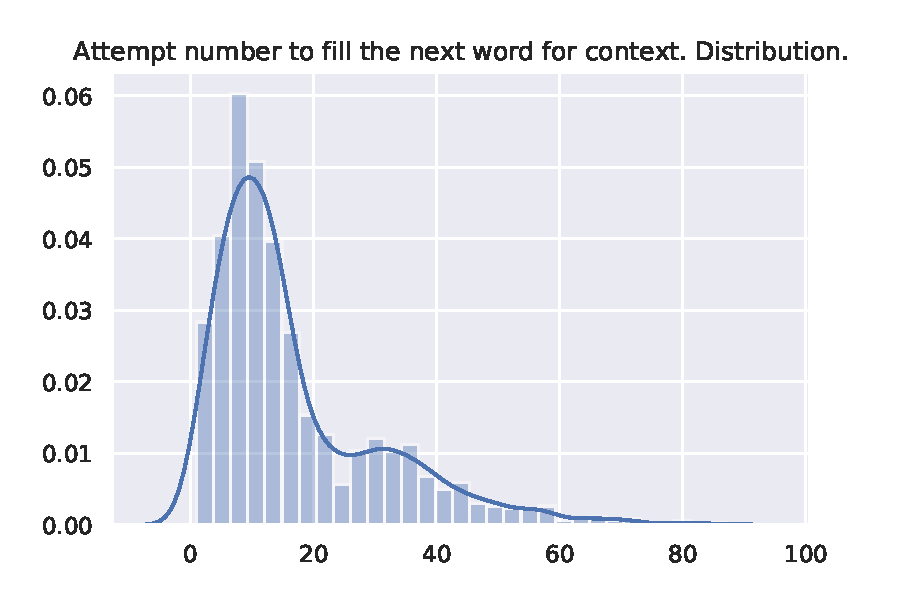
\includegraphics[width=0.4\textwidth]{figures/pdf/num-fill-context-dist.pdf}
\end{figure}
% TODO [ar]

\begin{table*}
\label{tbl:min-var}
\caption{Contexts in which minimum variance is observed in filling by
one lexical unit.}
\centering

\vspace{0.5em}

\begin{tabular}{l}
\begin{russian} Какие главные лекарства должны входить в\end{russian} \\
\begin{russian} В современном обществе семья и школа оказывают большое влияние\end{russian} \\
\begin{russian} Зачем ему звонить если откликается спокойный женский голос\end{russian} \\
\begin{russian} Ирине досталась отдельная комната в двухкомнатной квартире\end{russian} \\
\begin{russian} Они не ели целый день\end{russian} \\
\begin{russian} Во избежание ожогов надо нанести на лицо небольшое количество\end{russian} \\
\begin{russian} Во избежание ожогов надо нанести на лицо небольшое количество защитного крема\end{russian} \\
\begin{russian} Дрозды и скворцы начали вить семейные\end{russian} \\
\begin{russian} Дрозды и скворцы начали вить семейные гнезда неподалеку друг\end{russian} \\
\begin{russian} Дрозды и скворцы начали вить семейные гнезда неподалеку друг от друга\end{russian} \\
\begin{russian} Собаку виновницу случившегося приказали сечь хотя в чем была ее вина\end{russian} \\
\begin{russian} С нескрываемой едкой иронией отзываются они друг о\end{russian} \\
\begin{russian} С нескрываемой едкой иронией отзываются они друг о друге\end{russian} \\
\begin{russian} Олень бродил среди берез жевал талый снег и\end{russian} \\
\end{tabular}
\end{table*}

In Table~\ref{tbl:min-var}, contexts with minimum variance in filling
are listed. It is worth emphasizing that in all the above cases there
was no variance in respondents’ answers, i.e. all respondents gave the
same one answer for these contexts. What is more, this predicted word
was the original word from the corpus.

We classified these contexts based on their constraining ability
% TODO [as]
 and found out the following groups of com:

Semantically constraining contexts [contexts \#3, 4, 6, 7, 8, 9]

Syntactically constraining contexts [contexts \#1, 14]

Idiomatically constraining contexts [contexts \#2, 5, 10, 11, 12, 13]

The maximum number of different answers were received for the “на болотах” (“On the Swamps”) context - 87 words, which is explained by the absence of any limiting semantic properties of the context.

In this regard, the study of the artificial language model distribution is meaningless, as it will always be uniform, so as to say, the indicator for each context in similar histograms will be equal to the size of the vocabulary.

\begin{figure}
\caption{Context length vs. lexical accuracy.}
\centering

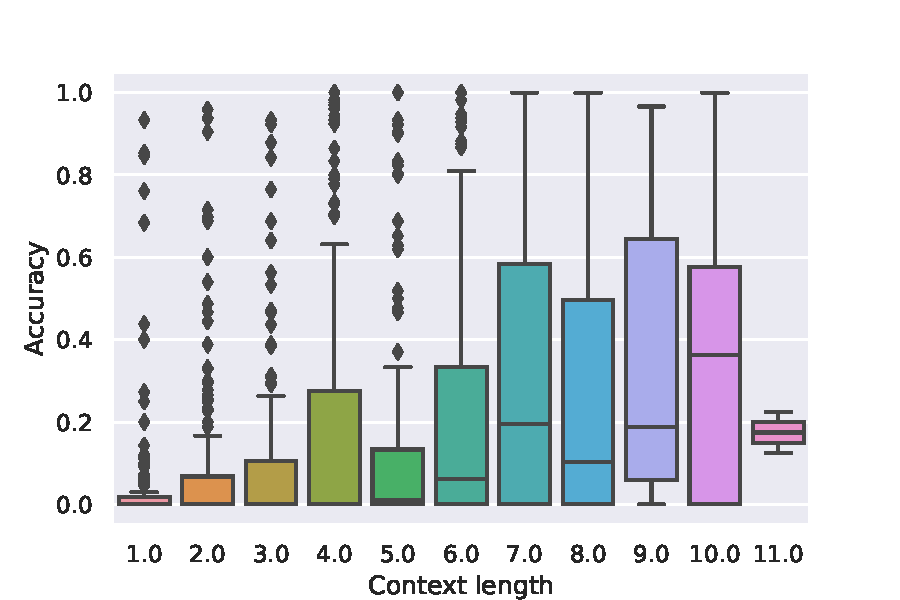
\includegraphics[width=0.4\textwidth]{figures/pdf/context-accuracy-lexical.pdf}

\end{figure}

Another important aspect in the study of the linguistic model of the cloze task is the relationship between the length of the context and the probability of predicting (=predictability of) the correct word.

In Figure~\ref{fig:context-accuracy-regression} reflects a high value of predictability for contexts of length both less and more than five lexical units. However, the lack of correlation is worth emphasizing. We received Pearson correlation coefficient score of 0.323 and Spearman correlation coefficient of 0.363.

According to the results of our experiment, the closest probability distribution of the correct word of all the models was achieved with BERT trained on the literary
% TODO [at]
 corpus.

In this case
% TODO [au]
, there is practically no correlation
% TODO [av]
: Pearson correlation score is 0.093521, Spearman correlation - 0.079094.

\begin{figure}
\label{fig:context-accuracy-regression}
\centering
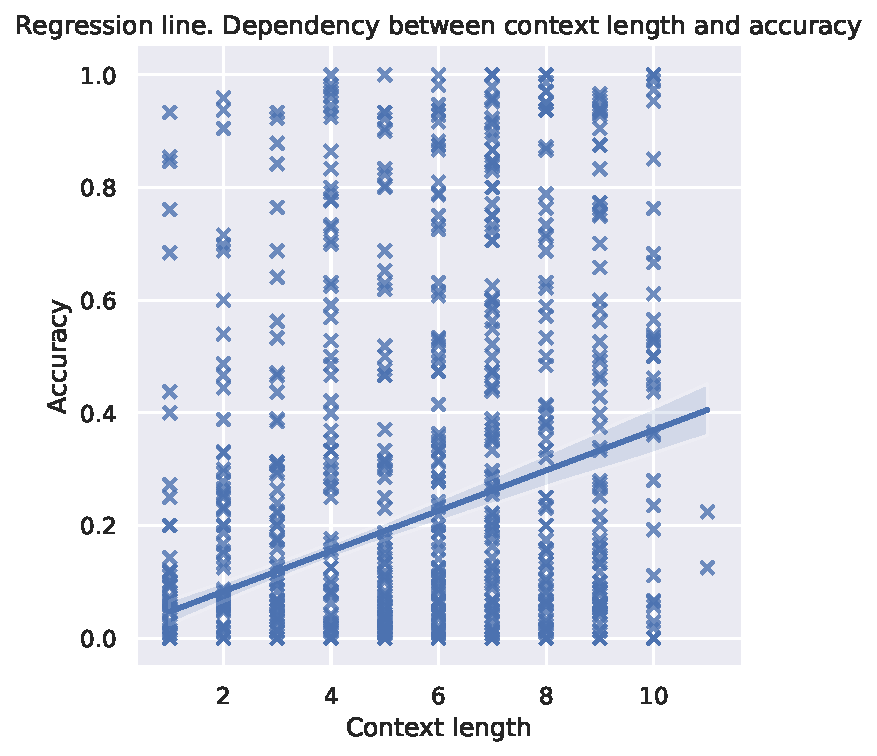
\includegraphics[width=0.4\textwidth]{figures/pdf/context-accuracy-regression.pdf}
\end{figure}

% TODO [aw]


Each model was evaluated by two measures: mean accuracy of model predictions and absolute number of correct word predictions. For computing mean accuracy, the mean of correct answer probabilities was taken. In case of absolute number of correct word predictions, a model achieved +1 score if there was at least one correct answer among all predictions.
% TODO [ax]


\subsection{Model comparison on the Lexical Level}

\head{Mean Accuracy}

Figure~\ref{fig:mean-accuracy-hist-lex}
% TODO [ay]
% TODO [az]
 below shows a bar chart of the mean accuracy scores of each model on
the lexical level. As the goal of our study was to build an algorithm,
which would be the closest approximation of the cloze task results
(18\% accuracy), we can see that BERT (not a language model one) model
scored better than the others. Interestingly, all HMM model
architectures showed low results on the lexical level.

\begin{figure}
\caption{Mean accuracy histogram, lexical level.}
\label{fig:mean-accuracy-hist-lex}
\centering
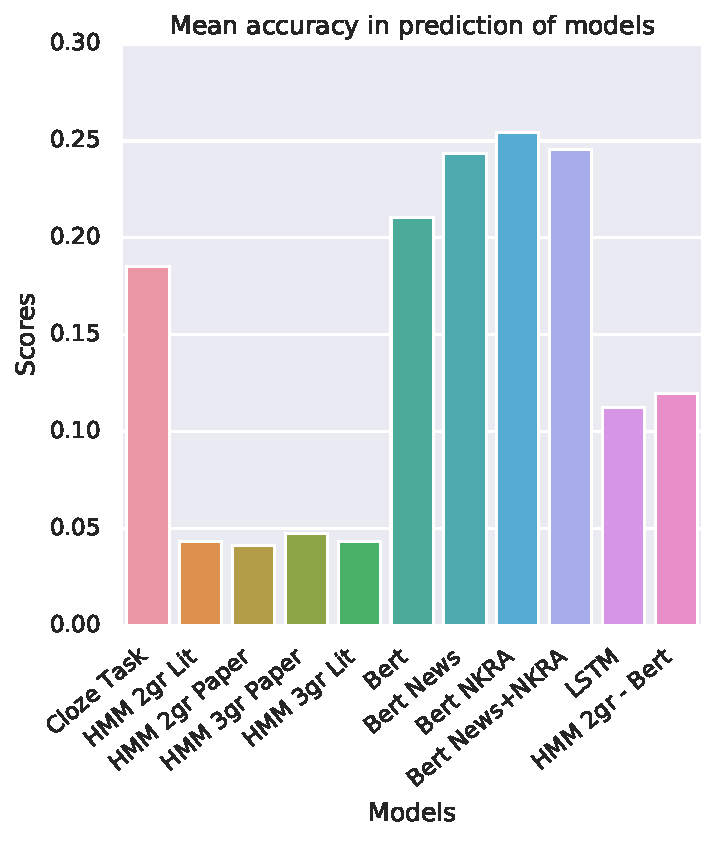
\includegraphics[width=0.4\textwidth]{figures/pdf/mean-accuracy-hist-lex.pdf}
\end{figure}

It is noticeable that BERT mean accuracy results are higher than cloze task score. This can be explained by the fact that the model was trained on a large amount of written texts and thus had a higher chance to guess the correct word. Following this assumption, an assumption can be made that respondents’ active vocabulary size is lower than model’s vocabulary. Also, we can make a hypothesis that the process of word retrieval by humans and by the model is performed differently, as respondents do not always respond with the most probable answer
% TODO [ba]
.

\head{Absolute Accuracy}

In terms of absolute number of predicted words, in the cloze task around 625 contexts were given at least one correct prediction. The closest to that are the results of the bigram HMM model combined with BERT (with around 545 contexts with at least one correct prediction) and raw BERT (with about 725 contexts with at least one correct prediction).

\begin{figure}
\caption{Absolute accuracy histogram, lexical level.}
\label{fig:abs-accuracy-hist-lex}
\centering
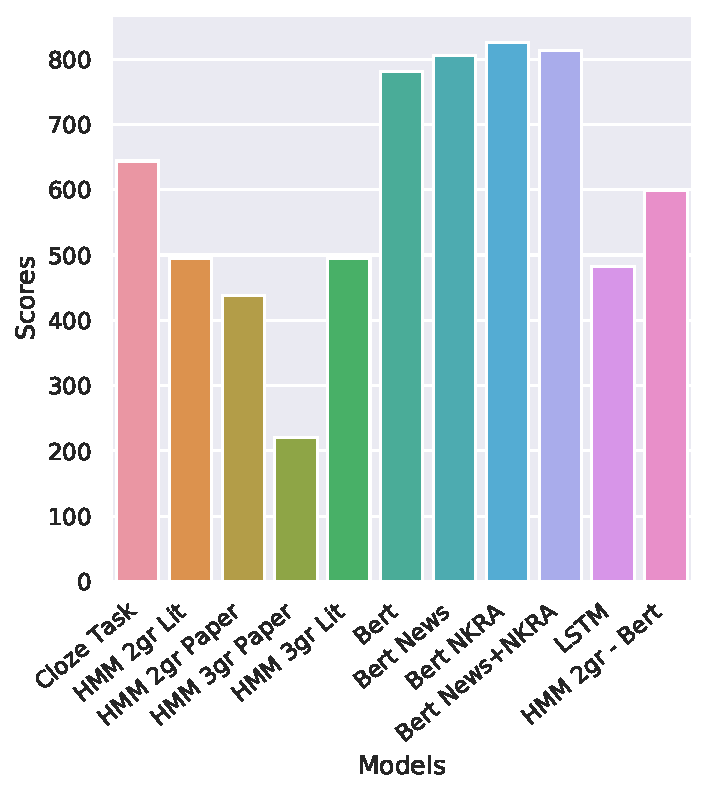
\includegraphics[width=0.4\textwidth]{figures/pdf/abs-accuracy-hist-lex.pdf}
\end{figure}

\head{Model Consistency}

Next, we compared models’ performances using an inclusion-exclusion principle to find a percentage of overlapping answers between different models. The result of this comparison is shown on the heat map below.

The heat map reflects information on pairwise model comparison,
however we are mainly interested in how close the models are to the
cloze task model. The comparison showed that the models with the
largest overlap with the cloze task are birgram HMM model combined
with BERT (58\% of overlap) and BERT trained on RNC.

\begin{figure}
\caption{Overlap heatmap, lexical level.}
\label{fig:heatmap-context-accord-lex}
\centering
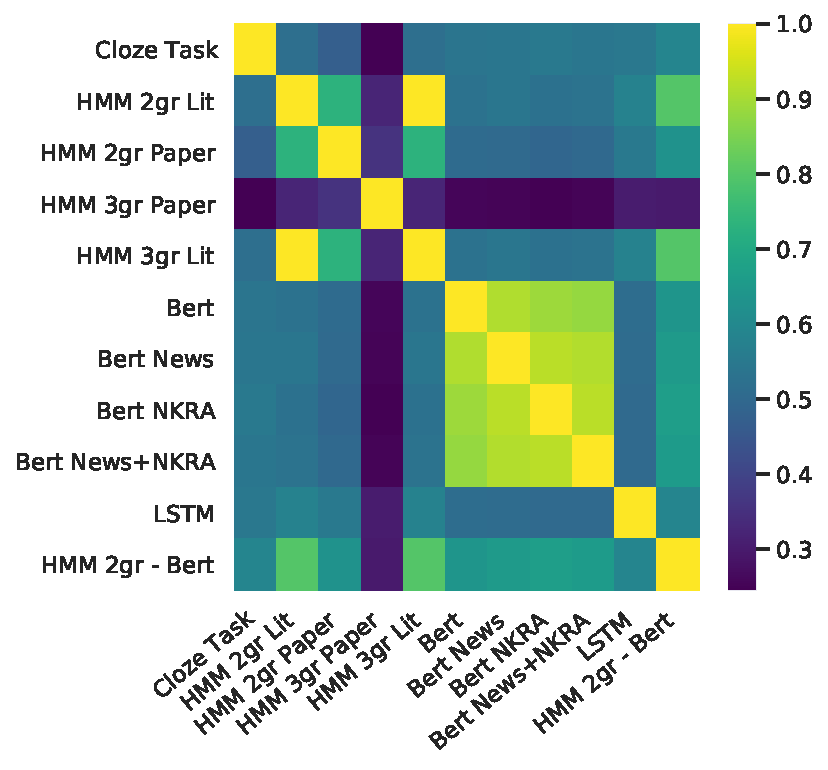
\includegraphics[width=0.4\textwidth]{figures/pdf/heatmap-context-accord-lex.pdf}
\end{figure}

\head{Kolmogorov-Smirnov}

At the next step, we performed Kolmogorov-Smirnov testing to find the similarity in the probability distributions of the model predictions. This table also reflects the sum value of pairwise comparison of the contexts using Kolmogorov-Smirnov testing. For convenience all the values were normalized. Observations show that the closest probability distribution is seen in LSTM model. However, as we see, there is a variation in metric values from 0.9 to 6.2 for different models. Thus, we can assert that the difference between all models and a cloze task is rather large and in some way unacceptable.
% TODO [bb]




%\head{Cosine Similarity}
%To measure model predictions on semantic level, the cosine similarity between each context’s predicted words centroid vector was found. The number of words was selected dynamically for each context by maximizing vector significance with the minimum words.
%

% TODO [bc]

\head{Kullback–Leibler divergence} % Sergey

Due to the fact that all of our models are word-level, and in order to lower the casing variability we've combined all our vocabularies into one
% TODO [bd]
. For this compound vocabulary we calculated the KL divergence of our models.

The table below shows the scores for three different models with
bigram HMM trained on NCRL showing the best results. Unfortunately,
this heat map does not show us changes in LM \{language model?\} distances context-lengthwise. Table of top-3 of lengthwise LM distances.

\begin{table}
\centering

\caption{KL scores for three different models, all trained on the
National Corpus of the Russian Language. ``Context provided'' is in number
of tokens.}

\begin{tabular}{rrrr}
\textbf{Context} &
\textbf{Bigram HMM} &
\textbf{BERT} &
\textbf{LSTM} \\
\hline
1 &
1.34 &
2.17 &
2.01 \\
2 &
1.57 &
2.10 &
1.78 \\
3 &
1.84 &
2.07 &
1.84 \\
4 &
1.79 &
1.93 &
1.81 \\
5 &
1.91 &
2.02 &
1.92 \\
6 &
1.86 &
1.88 &
1.87 \\
7 &
1.99 &
1.77 &
1.89 \\
8 &
1.73 &
1.69 &
1.80 \\
9 &
1.97 &
1.55 &
1.63 \\
10 &
2.46 &
1.71 &
1.80 \\
11 &
2.79 &
2.68 &
2.17
\end{tabular}
\end{table}

As we see, the bigram models starts to higher the distance from 1 to 6 context length, but BERT on the contrary start to lower the distance up to 6 context length. For this case we merged bigram model and BERT at border of length 6.
KL(Cloze || Cloze) = 0.0
KL(Cloze || HMM) = 1.79
KL(Cloze || BERT) = 1.93
KL(Cloze || LSTM) = 1.84
KL(Cloze || HMM + BERT) = 1.71

\subsection{Model comparison on the PoS level} % Semen, Anastasia

\head{Mean Accuracy}

The performance of all models, except for LSTM
% TODO [be]

% TODO [bf]

% TODO [bg]
, at the parts of speech level has significantly and proportionally increased. This is due to a decrease in the set of classes for which classification occurs. At this stage, the first 30 words of each model were tagged for parts of speech. Overall, there were 16 word classes. It is notable that BERT linguistic models have the highest scores.

\begin{figure}
\caption{Mean accuracy histogram, part-of-speech level.}
\label{fig:mean-accuracy-hist-pos}
\centering
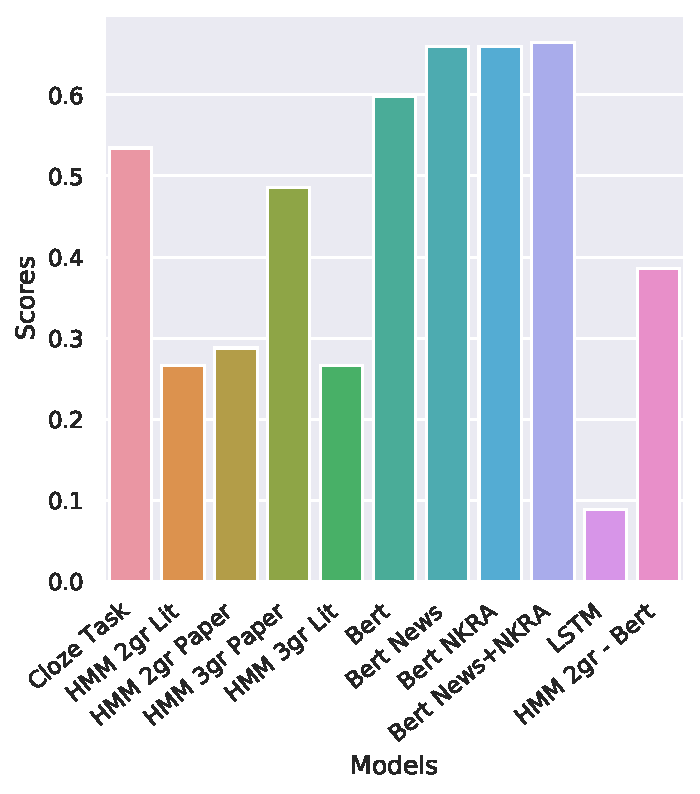
\includegraphics[width=0.4\textwidth]{figures/pdf/mean-accuracy-hist-pos.pdf}
\end{figure}



\head{Absolute Accuracy}

In absolute values, there is also a tendency in higher accuracy of BERT models, which can be interpreted as follows. BERT as a language model (lm) correctly predicts a part of the next word, but the words themselves, rather close to the context, have a low probability. Moreover, in many cases, they have almost a uniform distribution equal to 0.033.

\begin{figure}
\caption{Absolute accuracy histogram, part-of-speech level.}
\label{fig:abs-accuracy-hist-pos}
\centering
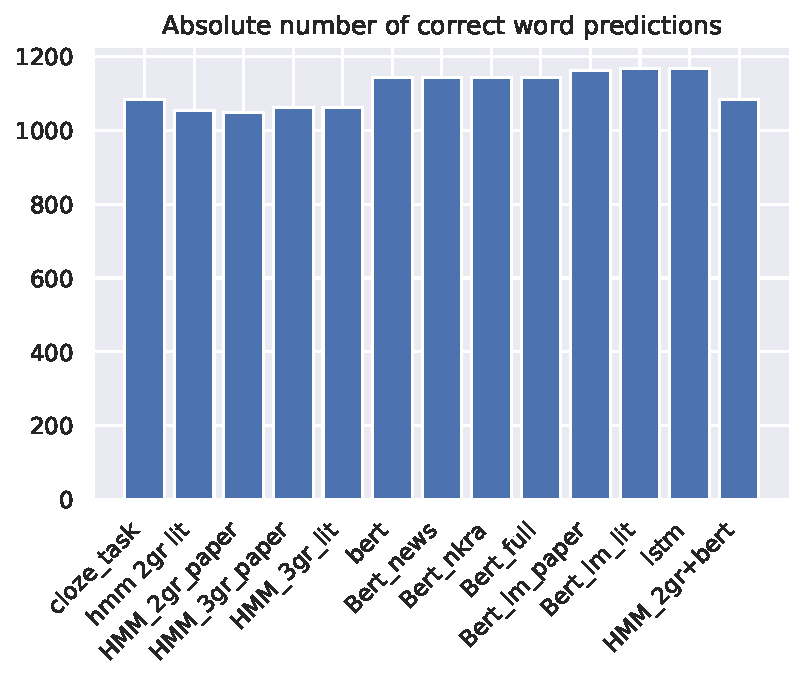
\includegraphics[width=0.4\textwidth]{figures/pdf/abs-accuracy-hist-pos.pdf}
\end{figure}


\head{Model Consistency}

The consistency of a part of speech prediction differs significantly from the lexical level. However, when compared with the cloze task model, we do not see a strong resemblance with one of the artificial models. That is, there are contexts for which a person is able to predict the part of speech of the next word correctly, while the models are not able to do the same.

\begin{figure}
\label{fig:heatmap-context-accord-pos}
\caption{Overlap heatmap, part-of-speech level.}
\centering
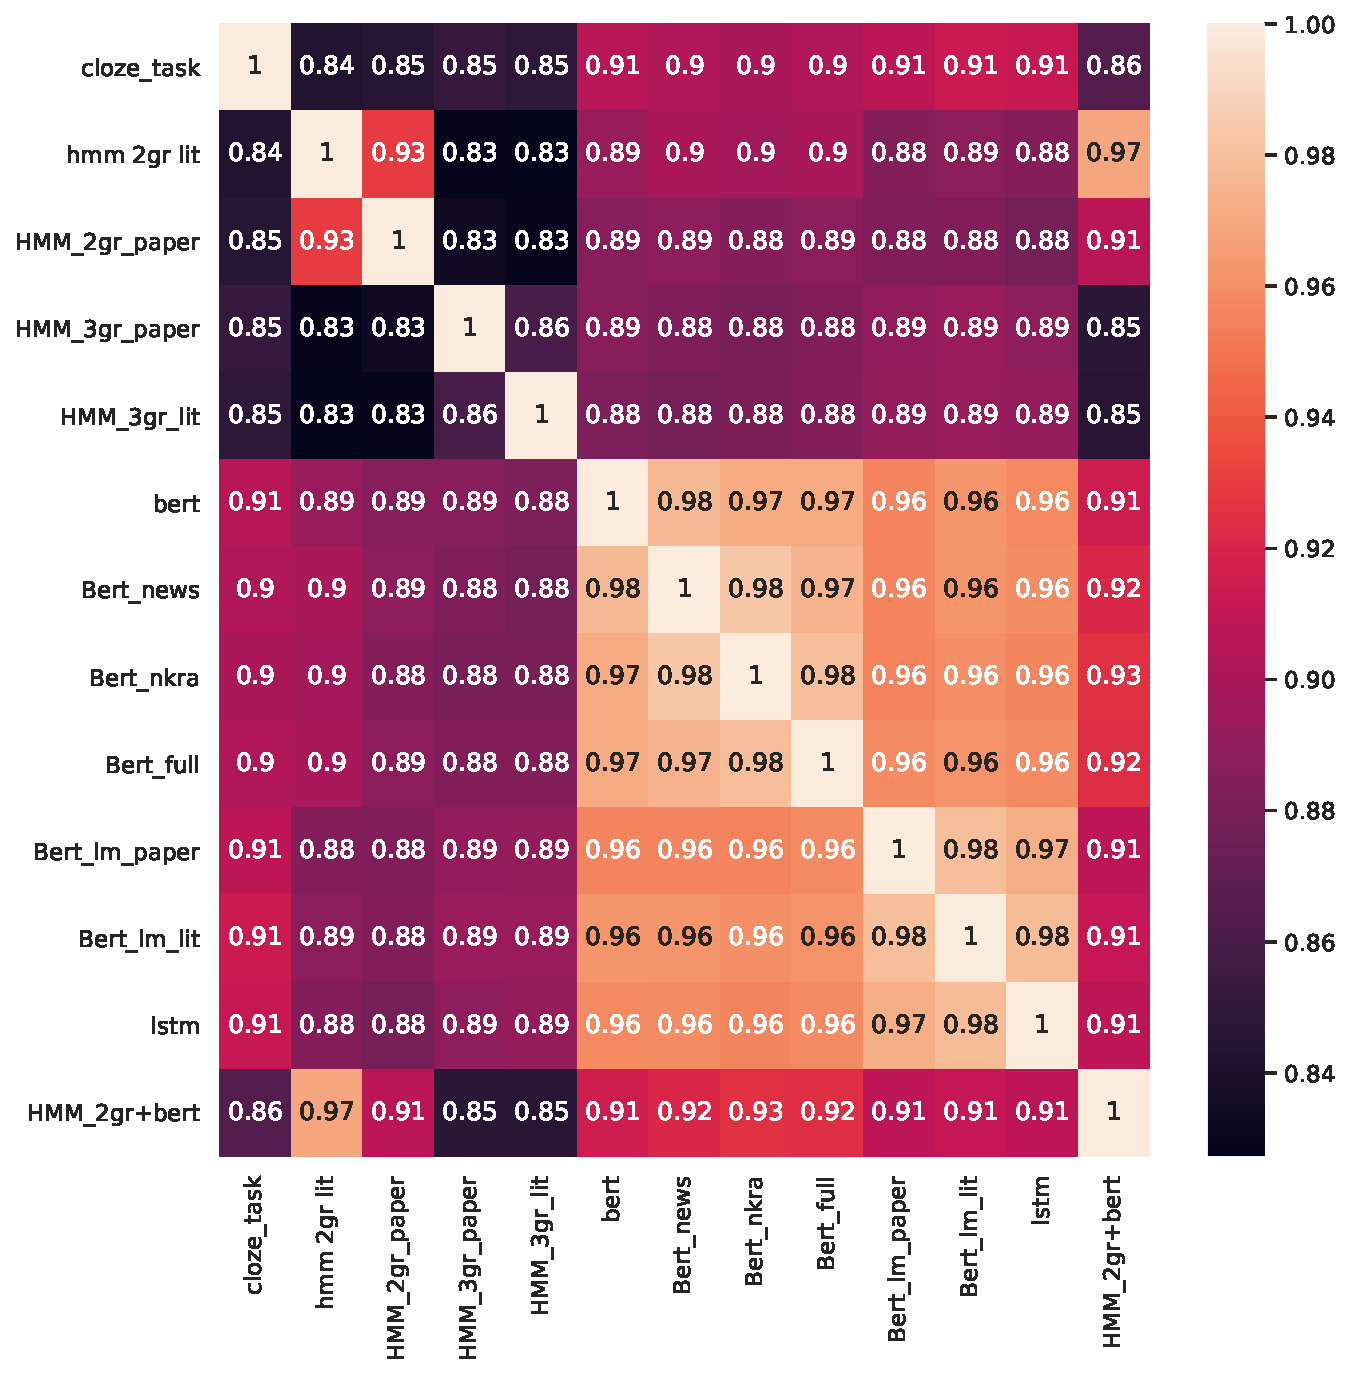
\includegraphics[width=0.4\textwidth]{figures/pdf/heatmap-context-accord-pos.pdf}
\end{figure}


\subsection{Model comparison on the OMVF level} %  Semen, Daria

\head{Mean Accuracy}

Reducing the number of classes by 4 times does not lead to an improvement in the average accuracy
% TODO [bh]
. Although we can see that the models perform similar as on the original parts of speech model.

\begin{figure}
\caption{Mean accuracy histogram, object-verb-functional-modifier level.}
\label{fig:mean-accuracy-hist-ovfm}
\centering
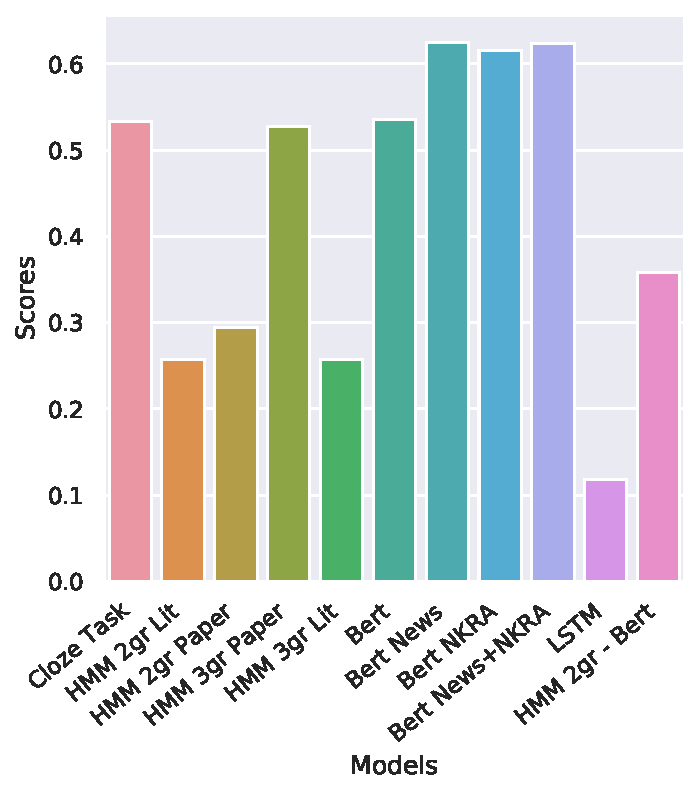
\includegraphics[width=0.4\textwidth]{figures/pdf/mean-accuracy-hist-ovfm.pdf}
\end{figure}


\head{Absolute Accuracy}

Absolute values at OMVF level of generalization cease to reflect
any properties of the models. This is due to the metric calculation
algorithm. The model's indicator increases by one each time when there
is a correct answer and its probability is not equal to 0.
Accordingly, the graph reflects that in more than 95\% of cases the
correct tag is present. It can be noted that for a model with a random
tag generator, this threshold would be 25\%. Such differences in magnitudes suggest productivity at the OMVF level. 

\begin{figure}
\caption{Absolute accuracy histogram, object-verb-functional-modifier level.}
\label{fig:abs-accuracy-hist-ovfm}
\centering
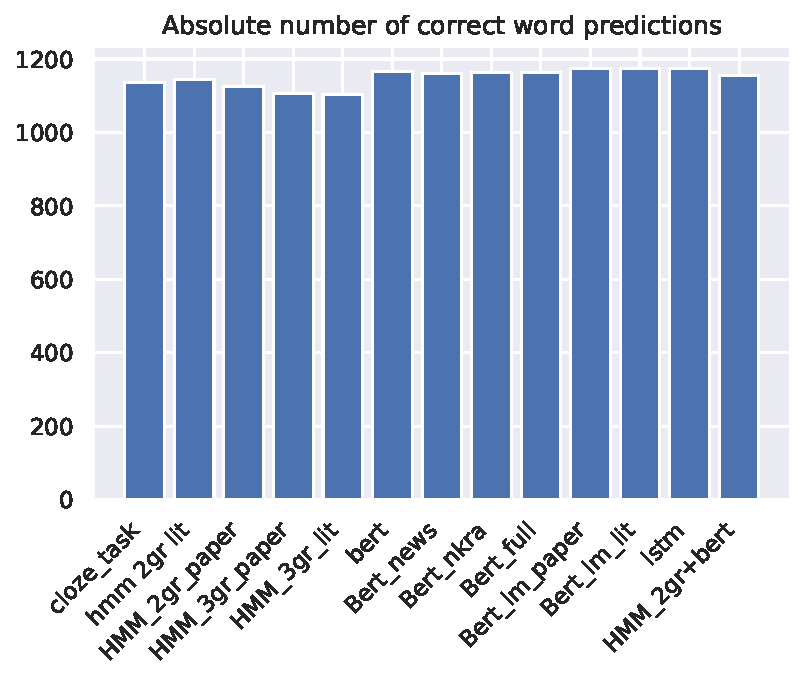
\includegraphics[width=0.4\textwidth]{figures/pdf/abs-accuracy-hist-ovfm.pdf}
\end{figure}

\head{Model Consistency}

Consistency at the object-verb-functional-modifier level is shown in
Figure~\ref{fig:heatmap-context-accord-ovfm}.

\begin{figure}
\label{fig:heatmap-context-accord-ovfm}
\caption{Overlap heatmap, object-verb-functional-modifier level.}
\centering
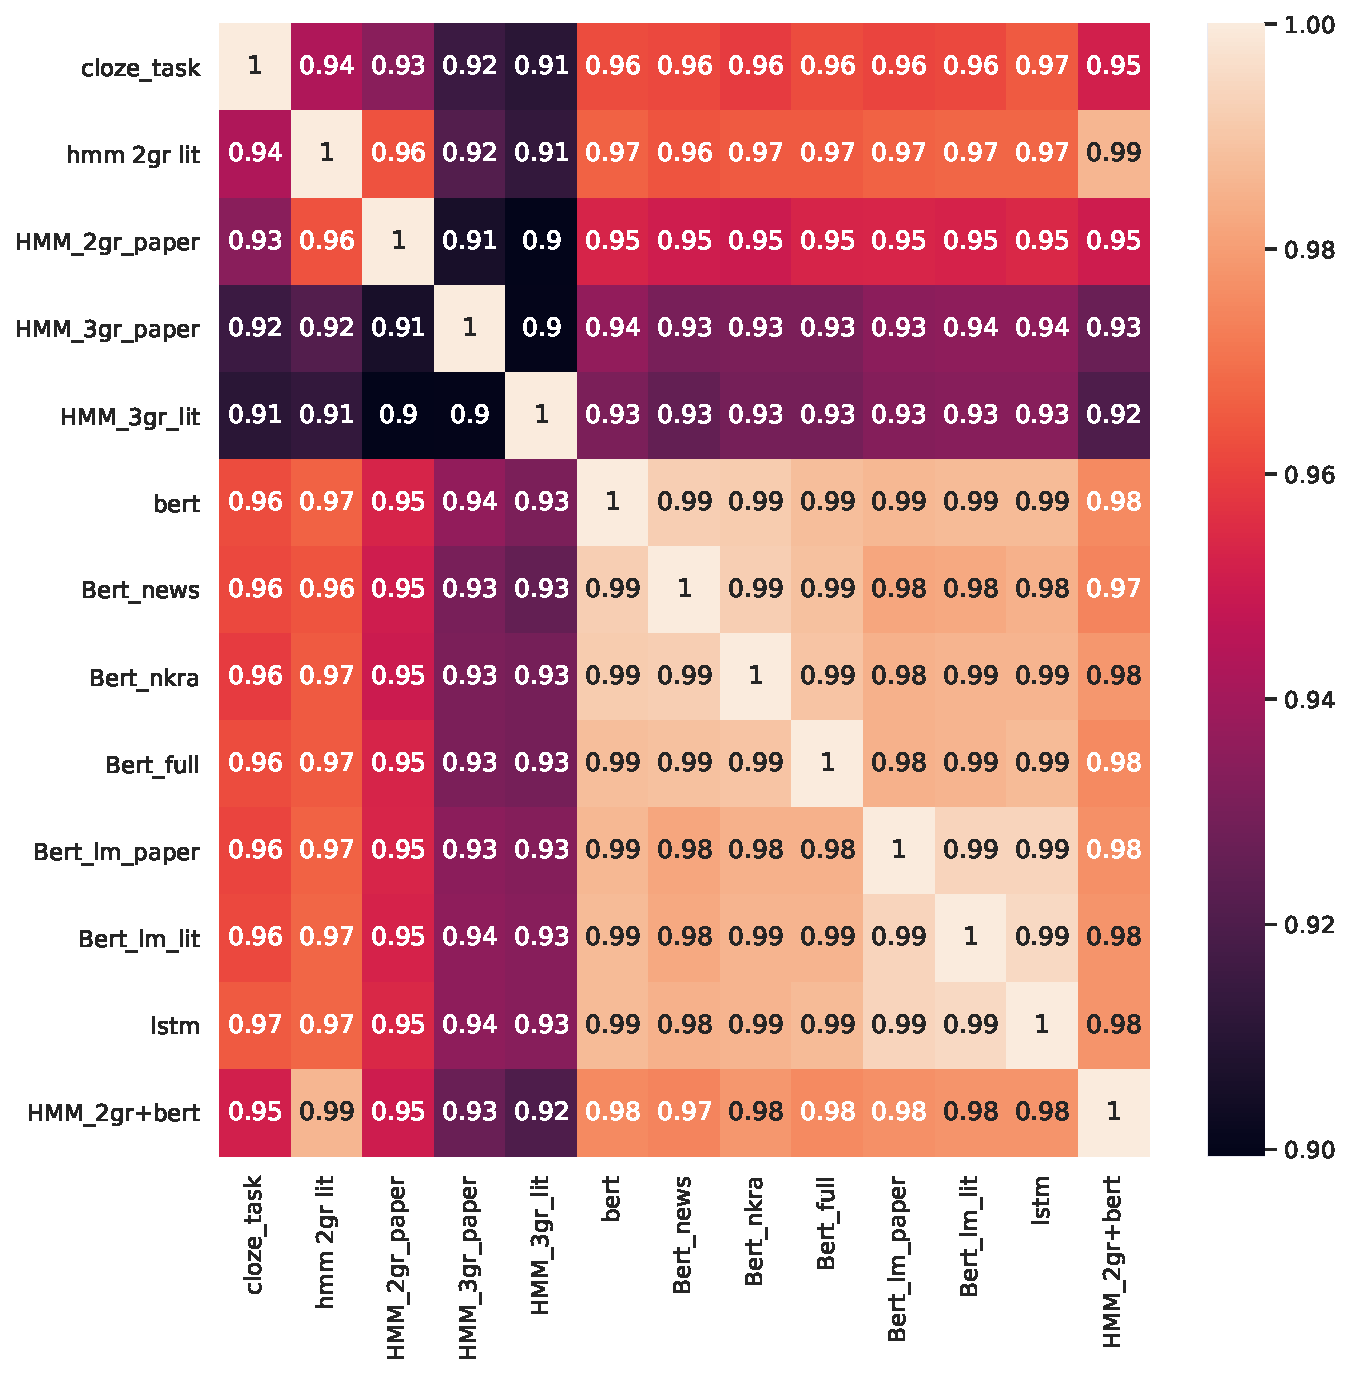
\includegraphics[width=0.4\textwidth]{figures/pdf/heatmap-context-accord-ovfm.pdf}
\end{figure}

\head{Kolmogorov-Smirnov}%KS test (based on absolute value statistics)

The last two tests reflect a contradictory trend: LSTM shows a greater resemblance to the cloze task. Here it is necessary to make a comment about probabilistic distribution. Calculation of statistical tests based on probability distributions of the models makes the metrics far from objective, since the variation of the number of lexical units to consider significantly impacts the final output. Thus the results may highly differ for 25 and 30 lexical units. Moreover, artificial models allow us to reflect distributions for the large vocabulary, whereas the vocabulary of the cloze task is very limited and has many random outliers when the context is not constraining the next word on any level. It is disputable whether such cases should be eliminated from the vocabulary during research or not.                          

\section{Conclusion}

\section{Bibliography}% [bi] 
\bibliographystyle{lrec}
\bibliography{paper}


\end{document}

% [a]no abstract
% 
% [b]it is very limited in the text
% 
% [c]it is not present in the text...
% 
% [d]task?
% 
% [e]not clear, how probability score is calculated
% 
% [f]??? can we measure predictability of a context?
% 
% [g]too strong
% 
% explains variance
% 
% [h]other papers show that it is not an oblagation
% 
% [i]incorrect implication
% 
% [j]does it?
% 
% [k]what is the rationale behind all these models?
% 
% Why did you choose them?
% 
% [l]not clear: how did you plan to retransform BERT?
% 
% [m]how this sentence is related to the previous one?
% 
% [n]Непонятно: в итоге BERT у вас видит контекст справа или нет?
% 
% [o]why did you select these particular corpora?
% 
% [p]link
% 
% [q]and what about later texts?
% 
% [r]what corpus it was trained on?
% 
% [s]trained on what?
% 
% [t]did you train your own lstm?
% 
% [u]why?
% 
% [v]add to the references
% 
% [w]how was it computed
% 
% [x]how was it computed
% 
% [y]how was it computed
% 
% [z]latex format for the final article
% 
% [aa]what is it? it was not introduced above
% 
% [ab]which of the models was a classification model? it was not explained above
% 
% [ac]unclear
% 
% [ad]what it the rationale to compute Pos probabilities?
% 
% [ae]PoS or word class? choose one nomination
% 
% [af]it is my text
% 
% [ag]did you do this for the cloze task responses?
% 
% [ah]references
% 
% [ai]did you do this for models' predictions or for cloze responses as well?
% 
% [aj]what did you try? can you list it?
% 
% [ak]what does it mean? what was the goal?
% 
% [al]why did you choose this model???
% 
% [am]какова идея за этой функцией? вы можете сначала объяснить, что вы в принципе хотели сделать?
% 
% [an]how did you get this number?
% 
% [ao]where? in the context?
% 
% [ap]in context?
% 
% [aq]for each context or for each word in context?
% 
% why did you measure semantic similarity of contexts?
% 
% [ar]number of guesses for each target word?
% 
% [as]More info on constraining contexts with reference to the original article
% 
% [at]which one?
% 
% [au]not clear
% 
% [av]between what and what?
% 
% [aw]do this figures illustrate BERT??
% 
% [ax]not clear
% 
% [ay]I am surprised with the lstm results
% 
% In our study we got 19% accuracy for lstm trained on the national corpus of Russian
% 
% [az]https://colab.research.google.com/drive/1vZ4a2T-cCpE76VGvw4E-IyODy7XapWkc Добрый день, здесь выложил часть кода, отвечающую за расчет метрики для ЛСТМ,  не могли бы сверить со своими результатами?
% 
% [ba]это довольно странное заключение: что мы считаем наиболее вероятным ответом? Что у нас является золотым стандартом вероятности ответа? Почему ответ BERT более вероятный, чем ответ людей?
% 
% [bb]why? what are the acceptability criteria?
% 
% [bc]what does the heatmap reflect?
% 
% [bd]why did you decide to do this?
% 
% [be]this is a really strange result
% 
% Can you double-check it?
% 
% [bf]and it contradicts your calculations below (3)
% 
% [bg]Непонятно, как PoS accuracy вообще может быть ниже word accuracy: если модель правильно предсказала слово, то она и его часть речи правильно предсказала.
% 
% [bh]this is also very strange
% 
% Are you absolutely sure about these results? How can you explain them?
% 
% [bi]should be aligned with the text

